\subsection{From vertex enumeration to convex hull}


In geometry, vertices and half-spaces are close concepts: a vertex $(a_i)_{i=0}^d$ can be associated to a half-space $\sum_{i=0}^d x_i a_i \leq 1$ and vice-versa. This association is the \emph{geometric duality} and it allows to use the vertex enumeration algorithm to find the convex hull of a polyhedron. The emptiness and the equality to a single point of a $\mathcal{V}$-polyhedron is trivial to check, in the following, the polyhedron and polytopes are assumed to be at least two-dimensional. Figure~\ref{ex_dual} shows a pair vertex/half-space and two triangles that are dual from each other.

\begin{figure}
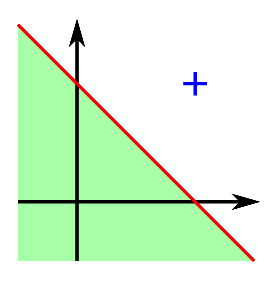
\includegraphics[scale=1]{images/dual.eps}
\hspace*{1cm}
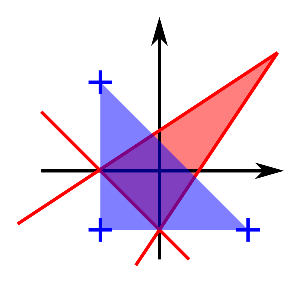
\includegraphics[scale=1]{images/dual4.eps}
\caption{Left: pair vertex/half-space that are dual from each other. Right: two triangles dual from each other.}
\label{ex_dual}
\vspace*{-0.7cm}
\end{figure}

\subsubsection{The convex hull of a polytope}
The polytope studied is refereed as $P$, convex hull of the set $V$. Even it means to translate $P$, it is assumed that $\sum_{x\in V} x = 0 $. Since the polytope is at least two-dimensional, the origin is not a vertex. 

\begin{definition}[The dual of a subset of $\mathbb{R}^d$]
The dual $P^\Delta$ of a subset $P$ of $\mathbb{R}^d$ is defined by $\{c | \forall x \in P, cx\leq 1  \}$
\end{definition}

Theorem~\ref{thm_dual} holds the idea of the transformation:

\begin{theorem}
If $P$ is a polytope and $0\in P$, $P=(P^\Delta)^\Delta$.
\label{thm_dual}
\end{theorem}

Starting with the set of the vertices of $P$, the algorithm begins by switching to $P^\Delta$, which is described by a set of half-spaces. The vertices of $P^\Delta$ enumerated and the dual is taken, which leads to a set of half-spaces describing $P$. Indicing by the description mean, the algorithm does $ P_V \rightarrow P_H^\Delta \rightarrow P_V^\Delta \rightarrow P_H^{\Delta\Delta} = P_H $. 

The first step ($P_V \rightarrow P_H^\Delta$) does not hold any problem and is done with Theorem~\ref{thm_conv_dual}:
\begin{theorem}
For $P$ the convex hull of a given set $V$ of vertices, $P^\Delta=\{c | \forall x \in V, cx\leq 1\}$.
\label{thm_conv_dual}
\end{theorem}
The second step ($P_H^\Delta \rightarrow P_V^\Delta$) is done by the vertex enumeration algorithm. 

The third ($P_V^\Delta \rightarrow P_H^{\Delta\Delta}$) does not cause any problem if the origin is not on a facet of $P$ (or a face of other dimension, seen as an intersection of facets): then $P^\Delta$ is bounded and Theorem~\ref{thm_conv_dual} holds.

Otherwise, let $\{x|w.x \leq 0\}$ be a facet of $P$ (since $0$ is the iso-barycenter of $P$, $\{x| -w.x \leq 0\}$ is also a facet). Let $x\in P$, $y\in P^\Delta$ and $\alpha\in\mathbb{R}$, $(y+\alpha w).x=y.x+\alpha(w.x)=y.x$, this means that $lineal(w)$ is a linealty space of $P^\Delta$. $P^\Delta=conv(V')+lineal(L')$ thus $P^{\Delta\Delta}=conv(V')^\Delta \cap L'^\bot$ by the proposition~\ref{prop_lineal_dual}. Which end the convex hull problem for a polytope.

\begin{proposition}
For $V$ a set of vertices and $L$ a set of non null vectors $(conv(V)+lineal(L))^\Delta = conv(V')^\Delta \cap L'^\bot$. 
\label{prop_lineal_dual}
\end{proposition}
\begin{proof}
Let $y\in (conv(V)+lineal(L))^\Delta$, for all $v\in V$, $l \in L$ and $\alpha\in\mathbb{R}$, $y.(v+\alpha l)\leq 1$. The inequality holding for any $\alpha$,  $y.l=0$ and $y.v\leq 1$ and $y\in conv(V')^\Delta \cap L'^\bot$. Conversely, let $y \in conv(V')^\Delta \cap L'^\bot$ which means $y.\alpha l=0$ and $y.v\leq 1$ thus $y.(v+\alpha l)\leq 1$ for all $v\in V$, $l \in L$ and $\alpha\in\mathbb{R}$: $y\in (conv(V)+lineal(L))^\Delta$.
\end{proof}

\paragraph{Complexity:} taking the dual of a polytope costs $O(n)$ if the object is not totally rewritten, even if rewritten it costs $O(nd)$. Either way, the cost of the convex hull problem is the cost of Fukuda's algorithm.

\subsubsection{The convex hull of a cone}\label{ss_conehull}
To find the convex hull of a cone $C$, the convex hull algorithm for a set of points is used.
The origin is added to the set of vectors describing the cone, as for all $c$ in $C$, the segment between the origin and $c$ must belong to the cone. Then the half-spaces for which  the constant is not zero (i.e. the origin does not saturate the constrain) are deleted. This deletion is required to ensure the unboundedness of the cone. Note that this method allows to handle a linealty direction as the sum of two vectors in the cone.

\subsubsection{The convex hull of a polyhedron}
Here the linealty space is injected in the cone (as the sum of two opposite vectors), as the treatment does not differ. Let $P=conv(V) + cone(C)$ be a polyhedron, the method is given by the following result:
\begin{proposition}
Let $P=conv(V) + cone(C)$ be a polyhedron, $C'$ the set obtained from $C$ by adding a $0$ as a $0^{th}$ coordinate to every vectors ($c \mapsto (0,c)$) and $V'$ the set obtained by, by adding a $1$ as a $0^{th}$ coordinate to every vectors ($v \mapsto (1,v)$), then $P=cone(V',C')\cap \{ x| x= (1,y), y\in \mathbb{R}^d \}$
\end{proposition}

Starting from $P$, $C'$ and $V'$ are easily obtained and $cone(V',C')$ is given in~\ref{ss_conehull}. The intersection is done as follows:
$$ \{ x\in \mathbb{R}^{d+1}| a_0x_0+\sum_{i=1}^da_ix_i\leq b\}\cap \{x|x_0=1\}=\{x\in \mathbb{R}^d|\sum_{i=1}^da_ix_i\leq b-a_0\}$$

This operation can generate half-spaces with an equation such as $0\leq b$, such half-spaces are those which does not intersect with $\{x|x_0=1\}$ and they are eliminated.

\paragraph{Complexity:} the cost of the convex hull in the unbounded case is the cost of Fukuda's algorithm with one more point and a dimension bigger by one.



